\documentclass{article}
\usepackage[left=2.5cm,right=2.5cm, top = 2.5cm, bottom = 3cm]{geometry}
\usepackage{graphicx}
\usepackage{natbib}
\usepackage{hyperref}
\usepackage{todonotes}
\usepackage{booktabs}



\begin{document}
% \SweaveOpts{concordance=TRUE}

\title{A bootstrap-based comparison of ILI intensity thresholds from the moving epidemic and WHO methods}
\author{Johannes Bracher, Jonas Littek}
\date{ \small
Karlsruhe Institute of Technology (KIT), Chair of Statistics and Econometrics}

\maketitle


\abstract{The moving epidemic method (MEM) and the WHO method are widely used approaches to determine intensity levels for seasonal influenza and influenza-like illness (ILI). They are conceptually similar, but differ in two aspects. Firstly, the MEM involves a log-transformation of incidence data, while the WHO method typically operates on the original scale of the data. Secondly, the MEM method by default uses more than one observation from each past season, with a fixed total number of observations to include. The WHO method, on the other side, uses only the single highest value from each season to determine peak intensity thresholds. We perform a simulation study to assess the impact of these choices on the resulting intensity thresholds and empirical exceedance proportions. It is based on a bootstrap approach using historical ILI data from France, Spain, Switzerland and the United States. Using data on their original scale led to a too large proportion of seasons being classified as ``very high intensity'', which could to some degree be mitigated by using a logarithmic transformation. When fixing the total number of observations to include as in the MEM, intensity thresholds tend to increase as more data accumulates. When data is only available for few seasons, there is a rather large chance of classifying a new season as ``high'' or ``very high'' intenstity. We therefore advocate always using one observation per season with a log transformation, i.e.\ a hybrid between the default settings of the MEM and WHO methods.}

\section{Introduction}

Following the 2009 influenza H1N1 pandemic, the need for a rapid assessment tool for influenza intensity was recognized. In a report, the Review Committee on the Functioning of the
International Health Regulations and on Pandemic Influenza (H1N1) recommended that member states apply and evaluate their methods for severity assessment every year, thus improving their pandemic preparedness \citep[118]{WHO2011}. In the subsequent WHO Pandemic Infuenza Severity Assessment (PISA) guideline (\citeyear{WHO2017}), two specific statistical methods are recommended to determine influenza intensity thresholds. Firstly, the so-called \textit{WHO method}, already described in a previous document \citep{WHO2014} and in more detail in the PISA guide; and secondly, the \textit{moving epidemic method} (MEM) \citep{Vega2013, Vega2015} which is also recommended by the European Centre for Disease Prevention and Control (e.g.\ \citealt{ECDC2017}).

In particular the MEM approach has in the meantime been adopted by numerous national public health agencies (see references in Section \ref{sec:recent_applications}) and seems to deliver practically useful thresholds. The statistical properties of the MEM and WHO methods, however, have not yet been studied in detail. While it seems challenging to obtain strong mathematical results on their behaviour, we argue that simulation experiments can improve our understanding and intuition of the consequences of different implementation choices. We here provide such a simulation study, which in order to ensure a close link to real influenza patterns, is based on bootstrapping of historical surveillance data.

The article is structured as follows. Section \ref{sec:definitions} provides concise definitions of the MEM and WHO methods, highlighting two important differences between these conceptually similar approaches. Section \ref{sec:recent_applications} consists of an overview of published applications of the MEM and WHO methods. In Section \ref{sec:simulation} we describe our simulation approach and the results based on historical data from France, Spain, Switzerland and the United States. Section \ref{sec:discussion} concludes with a discussion.

\section{Definition of the moving epidemic and WHO methods}
\label{sec:definitions}

In the following we focus on the construction of thresholds  for peak intensity, framing the MEM and WHO methods as different special cases of the same general approach. Details on the construction of baseline thresholds from pre-season observations are omitted. We assume that thresholds are based on data from $n$ past seasons and applied to the ($n + 1$)-th season. \cite{Vega2015} recommend to use $5 \leq n \leq 10$ seasons for the MEM to ensure a sufficiently large, but recent data basis. Thresholds for for a given intensity measure $X$ are then obtained via the following steps:

\begin{enumerate}
\item Within each historical season order all observations, denoting the $i$-th largest observation from season $j$ by $X^{(i)}_j$.
\item Select the $K$ largest observations from each of the $n$ past seasons to construct a reference set $\mathcal{X} = \{X_j^{(i)}; j = 1, \dots, n; i = 1, \dots, K\}$.
\item Apply an (inversible) transformation $Y_j^{(i)} = f(X_j^{(i)})$ to all members of the reference set to obtain a reference set $\mathcal{Y}$ of transformed historical observations.
\item Assume that the transformed values in $\mathcal{Y}$ come from a normal distribution and compute estimates $\hat\mu, \hat \sigma$ of its mean and standard deviation.
\item Define intensity thresholds on the transformed scale as quantiles of the normal distribution N$(\hat\mu, \hat\sigma^2)$. A common choice for both methods \citep{WHO2017}, also implemented as the default in the \texttt{R} package \texttt{mem} \citep{Lozano2020} is
\begin{itemize}
\item the 40th percentile $q_{Y, 0.4} = \hat\mu - 0.25 \hat\sigma$ as the threshold between low and medium intensity;
\item the 90th percentile $q_{Y, 0.9} = \hat\mu + 1.28 \hat\sigma$ as the threshold between medium and high intensity;
\item the 97.5th percentile $q_{Y, 0.975} = \hat\mu + 1.96\hat\sigma$ as the threshold between high and very high intensity.
\end{itemize}
\item Obtain thresholds on the original scale by applying the inverse transformation, i.e. setting $q_{0.4} = f^{-1}(q_{Y, 0.4})$, $q_{0.9} = f^{-1}(q_{Y, 0.9})$, $q_{0.975} = f^{-1}(q_{Y, 0.975})$.
\end{enumerate}

\noindent The MEM and WHO methods are special cases of this procedure with the following specifications:
\begin{itemize}
\item In the MEM method, $f$ is chosen as the natural logarithm, while the number of observations per season is set to $K = 30/n$. (The exact specification used in the \texttt{R} package \texttt{mem} is $K = \max(1, \lfloor 30/n \rceil)$, where $\lfloor \cdot \rceil$ denotes rounding to the nearest integer.) The total number of historical observations is thus kept (approximately) fixed.
\item In the WHO method, the standard procedure is to set $f$ to the identity function (i.e.\ no transformation is applied). If peaks vary considerably, a log-tranformation is recommended \citep{WHO2017}. Irrespective of the number $n$ of historical seasons, $K = 1$ observation per season is used.
\end{itemize} 

\noindent The rationale of this approach is that ``about 50--60\% of the season peaks should be above the moderate threshold, $\pm 10\%$ above the high threshold and $\pm 2.5\%$ above the extraordinary threshold'' \citep{WHO2017}. Note that in most previous descriptions (e.g., \ \citealt{WHO2014, Vega2015}), the thresholds have been referred to as upper ends of one-sided confidence intervals associated with the the arithmetic (WHO method) or geometric mean (MEM) of the historical reference observations in $\mathcal{X}$. This, however, is slightly imprecise terminology as in the computations $\hat\sigma$ rather than $\hat\sigma/\sqrt{nK}$ is used. If indeed confidence intervals were used, these would tend to get narrower the more historical seasons were available, and the thresholds for all levels would eventually converge to the arithmetic / geometric mean. This is obviously not the intended behaviour.

% see function iconfianza.aritmetica

\section{An overview of recent applications}
\label{sec:recent_applications}

To get a better understanding of the different settings in which the MEM and WHO methods are applied in practice we performed a literature search among all published articles citing the papers \cite{Vega2015}, \cite{WHO2014} and \cite{WHO2017} until December 2020 (identified via \textit{CrossRef} and \textit{Google Scholar}). The results are summarized in Table \ref{tab:literature}. As can be seen from the numerous entries from the years 2019 and 2020, the MEM has quickly become a standard approach in the determination of intensity thresholds for influenza and other respiratory diseases. Indeed, the contributions come from numerous countries and in many cases have been co-authored by representatives of national or regional public health agencies. In most analyses, the suggested threshold levels at the 40th, 90th and 97.5th percentile are used. Variability with respect to the number $n$ of historical seasons included is considerable, with a range from 3 to 16 seasons. Consequently, the number $K$ of observations included per season ranges from two to ten. We only found few applications of the WHO methods, one of them providing a comparison to the thresholds from the MEM method \citep{Rguig2020}.

\begin{table}
\caption{Applications of the moving epidemic method and WHO method to determie severity thresholds. Does not contain works where only baseline thresholds are computed. The number of seasons included to compute thresholds is denoted by $n$, the number of observations used per season by $K$. Abbreviations: SARI = severe acute respiratory infection; ILI = influenza-like illness; RSV = respiratory syncytial virus.}
\label{tab:literature}
\center
\footnotesize
\begin{tabular}{l l l l l l l}
\multicolumn{7}{c}{(a) Moving epidemic method}\\ \\

\toprule
region & disease & years covered & $n$ & $K$ & percentiles & authors\\
\midrule
Australia & ILI/influenza & 2012--2017 & 5 & 6 & 40, 90, 99 & \cite{Vette2018}\\
Australia, Chile, & ILI/SARI & 2013--2019 & 6 & 5 & 40, 90, 97.5 & \cite{Sullivan2019}\\
New Zealand,\\
South Africa\\
Catalonia & ILI & 2010--2016 & 5 & 6 & ? & \cite{Basile2018}\\
Catalonia & ILI & 2005--2018 & 12 & 3 & ? & \cite{Basile2019}\\
Catalonia & ILI/influenza & 2010--2017 & 7 & 4 & ? & \cite{Torner2019}\\
Egypt & SARI/ILI & 2010--2017 & 6 & 5 & 40, 90, 97.5 & \cite{AbdElGawad2020}\\
Egypt & SARI & 2013--2015 & 3 & 10 & ? & \cite{Elhakim2019}\\
England & ILI & 2010--2016 & 6 & 5 & ? & \cite{Wagner2018}\\
Finland & influenza & 2011--2016 & 5 & 6 & ? & \cite{Pesaelae2019}\\
Montenegro & ILI & 2010--2018 & 7 & 4 & 40, 90, 97.5 & \cite{Rakocevic2019}\\
Morocco & ILI & 2005--2017 & 11 & 3 & 40, 90, 97.5 & \cite{Rguig2020}\\
Netherlands & RSV & 2005--2017 & 12 & 3 & 40, 90, 97.5 & \cite{Vos2019}\\
Norway & influenza & 2006--2015 & 9 & 3 & ? & \cite{Benedetti2019}\\
Pakistan & ILI, SARI & 2008--2017 & 10 & 3 & 40, 90, 97.5 & \cite{Nisar2020}\\
Portugal & ILI & 2012--2017 & 5 & 6 & 40, 90, 97.5 & \cite{Pascoa2018}\\
Scotland & influenza & 2010--2018 & 7 & 4 & ? & \cite{Murray2018}\\
Slovenia & RSV & 2008--2018 & 10 & 3 & 40, 90, 97.5 & \cite{Grilc2020}\\
Spain (17 regions) & ILI & 2003--2015 & 4--10 & 3--8 & 40, 90, 97.5 & \cite{Bangert2017}\\
Spain & ILI & 2001--2018 & 16 & 2 & 40, 90, 97.5 & \cite{RedondoBravo2020}\\
Tunisia & ILI & 2009-2018 & 9 & 3 & 50, 90, 95 & \cite{Bouguerra2020}\\
United Kingdom & ILI & 2000--2013 & 10 & 3 & 40, 90, 97.5 & \cite{Green2015}\\
United Kingdom & ILI/RSV & 2011--2018 & 4--6 & 5--8 & 40, 90, 97.5 & \cite{Harcourt2019}\\
USA & ILI/influenza & 2003--2015 & 11 & 3 & 50, 90, 98 & \cite{Biggerstaff2017}\\
USA & ILI & 2010--2015 & 5 & 6 & 50, 90, 98 & \cite{Dahlgren2018}\\
USA & influenza & 2010--2016 & 6 & 5 & 50, 90, 98 & \cite{Dahlgren2019}\\
\bottomrule\\
\multicolumn{7}{c}{(b) WHO method}\\ \\
\toprule
region & disease & years covered & $n$ & $K$ & percentiles & authors\\
\midrule
Cambodia & ILI & 2009--2015 & 7 & 1 & mean, 90, 95 & \cite{Ly2017}\\
Morocco & ILI & 2005--2017 & 11 & 1 & 40, 90, 97.5 & \cite{Rguig2020}\\
Philippines & ILI & 2006--2012 & 7 & 1 & 90 & \cite{Lucero2016}\\
Victoria/Australia & ILI & 2002--2011 & 6--10 & 1 & 90, 95 & \cite{Tay2013}\\
\end{tabular}
\end{table}

% Cite Benedetti who use it as a "gold standard". Mention Green GB who compare to percentile method. Vos mention fixed criterion model -- what is that?



\section{Simulaton study}
\label{sec:simulation}

\subsection{Goal}
\label{subsec:simulation_goal}

As detailed in the previous section, the MEM and WHO methods have been applied extensively in practice and overall seem to produce thresholds which are considered useful by domain experts. A more statistical assessment, however has so far been missing. We perform a simulation study to compare four versions of the general approach described in Section \ref{sec:definitions}:
\begin{enumerate}
\item[(a)] No transformation, $K = 1$. This corresponds to the WHO method.
\item[(b)] No transformation, $K = 30/n$.
\item[(c)] Logarithmic transformation, $K = 1$.
\item[(d)] Logarithmic transformation, $K = 30/n$. This corresponds to the default settings of the MEM approach.
\end{enumerate}

Our main focus is on the average share of seasons classified as low, medium, high and very high. As mentioned before, the medium, high and extraordinary threholds should be exceeded by approximately 60\%, 10\% and 2.5\% respectively \citep{WHO2017}. Concerning the choice between an identity and logarithmic transformation -- or, equivalently, the choice between arithmetic and geometric mean -- one may expect that the logarithm is more appropriate if observations are skewed. Concerning the number of observations used per available season, the choice $K = 30/n$ has the advantage of ensuring a reasonably large number of reference observations. However, this comes at the price of using observations which are not actually from peak weeks, and will by definition be lower than the actual peeks. If $n$ is low, this may lead to too low thresholds and a larger number of seasons classified as high or very high intensity. We will assess empirically whether such an effect can be observed, and how pronounced it is depending on the number of available historical seasons.

\subsection{Bootstrap approach based on historical ILI data}

A pure simulation study requires careful specification of a data-generating process mimicking the seasonal patterns of influenza. Given the considerable variability in timing and intensity of season peaks, this is not a trivial task. We therefore resort to a bootstrap approach based on historical data rather than generating synthetic data. Assume we have $N$ years of historical data on a measure of influenza activity. We then repeat the following steps a total of 500 times:

\begin{itemize}
\item Sample an ordered sequence of 15 seasons from the $N$ available seasons. As commonly done in bootstrap experiments, this is done with equal probability for each season and \textit{with replacement}, meaning that the same season can appear more than once in the sampled sequence. This approach is also referred to as the \textit{seasonal block bootstrap} \citep{Politis2001}.
\item For each value $n = 5, \dots, 15$:
\begin{itemize}
\item Restrict the generated sequence to the first $n$ seasons.
\item Apply approaches (a)--(d) as described in the previous subsection. Compute and store intensity thresholds for medium (40th percentile), high (90th percentile) and very high intensity (97.5th percentile).
\item Compute which fraction of the $N$ available seasons would be classified as low, moderate, high and very high using the obtained thresholds.
\end{itemize}
\end{itemize}
We can then assess how the thresholds and shares of the different intensity levels depend on the employed transformation function, the number of observations $K$ used per season and the number $n$ of seasons included.

\subsection{Data}

We use publicly available influenza surveillance data from four countries. Data on the weekly incidence of influenza-like-illness in France, 1985--2019, were obtained from the Réseau Sentinelles web platform (INSERM/Sorbonne Université, \url{https://www.sentiweb.fr}, \citealt{Flahault2006}). Population data were obtained from Institut national de la statistique et des études économiques. Data on weekly confirmed influenza cases in Spain, 1998--2019, were extracted from graphs shown in the \textit{Informe Anual} of the \textit{Sistema de la vigilancia de gripe en Espa\~na} (\url{https://vgripe.isciii.es/}; \citealt{SVGE2019}) using the tool \textit{WebPlotDigitizer} (\url{https://apps.automeris.io/wpd/}). Weekly ILI counts from Swiss routine surveillance, collected by the Swiss Federal Office of Public Health, 2000--2016, were obtained from the R package \texttt{HIDDA.forecasting} \citep{Held2019}. Population data were obtained from the Swiss Federal Statistical Office. Weekly weighted ILI percentage rates (wILI; corresponding to the percentage of general practitioner visits due to influenza-like symptoms) in the US, 1998--2017, from CDC FluView \cite{Charbonneau2019} were obtained from the CDC FluSight influenza forecasting platform (\url{https://github.com/FluSightNetwork/cdc-flusight-ensemble/}). 

All four time series are displayed in Figure \ref{fig:data}. Note that we removed the pandemic 2009/2010 influenza season from each series as it is not comparable to the usual years with only seasonal influenza. We also show boxplots of the first through sixth largest observation per season (right column). In the notation introduced in Section \ref{sec:definitions}, the first boxplot thus shows observations $X_j^{(1)}, j = 1, \dots, N$, the second $X_j^{(2)}, j = 1, \dots, N$ and so on. Little surprisingly (and by definition), the value get smaller on average for increasing ranks. Interestingly, they also get less dispersed, meaning that the variability between e.g.\ the sixth largest observations of the different seasons is always much smaller than that of the largest observations. 

% mention exact definition, source, number of seasons

\begin{figure}
\center
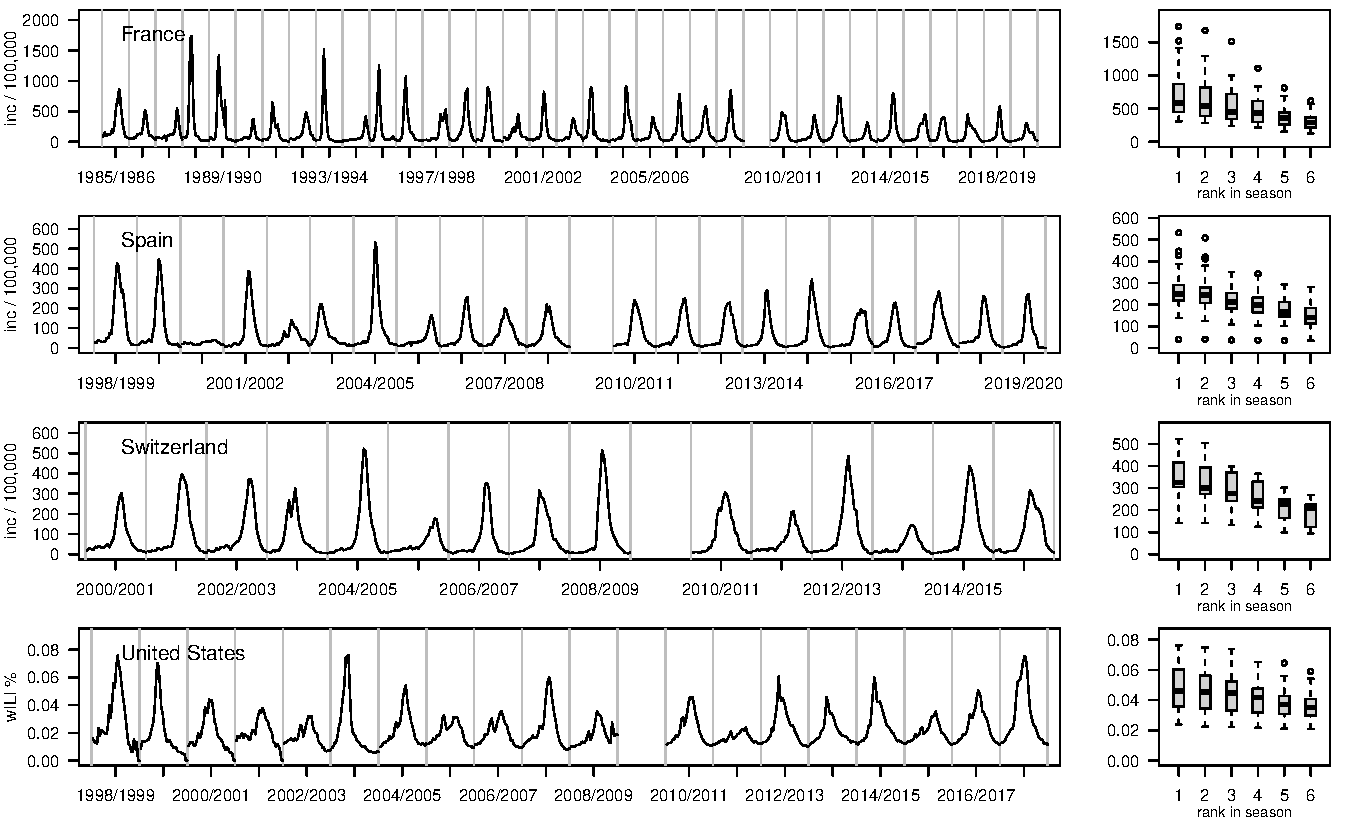
\includegraphics[width=0.9\textwidth]{figure/plot_data.pdf}
\caption{Time series of influenza activity measures in four countries: Weekly ILI cases per 100,000 population in France, 1985--2019; weekly number of confirmed influenza cases per 100,000 population in Spain, 1998--2019; weekly ILI cases per 100,000 in Switzerland, 2000--2016; weekly wILI percentages in the United States, 1998--2017.}
\label{fig:data}
\end{figure}

\subsection{Used software}

All of the following analyses were performed using the R language for statistical computing, version 4.0.3 \citep{RCT2020}, particular using the package \texttt{mem}, version 2.16 \cite{Lozano2020}. Note that the function \texttt{mem::memmodel} provides sufficient flexibility to apply all four approaches (a)--(d) from Section \ref{subsec:simulation_goal}. \todo{check whether app allows to change settings.}

\subsection{Results}

Results from our bootstrap simulation study for the four considered countries are shown in Figures \ref{fig:results1} and \ref{fig:results2}

\begin{figure}
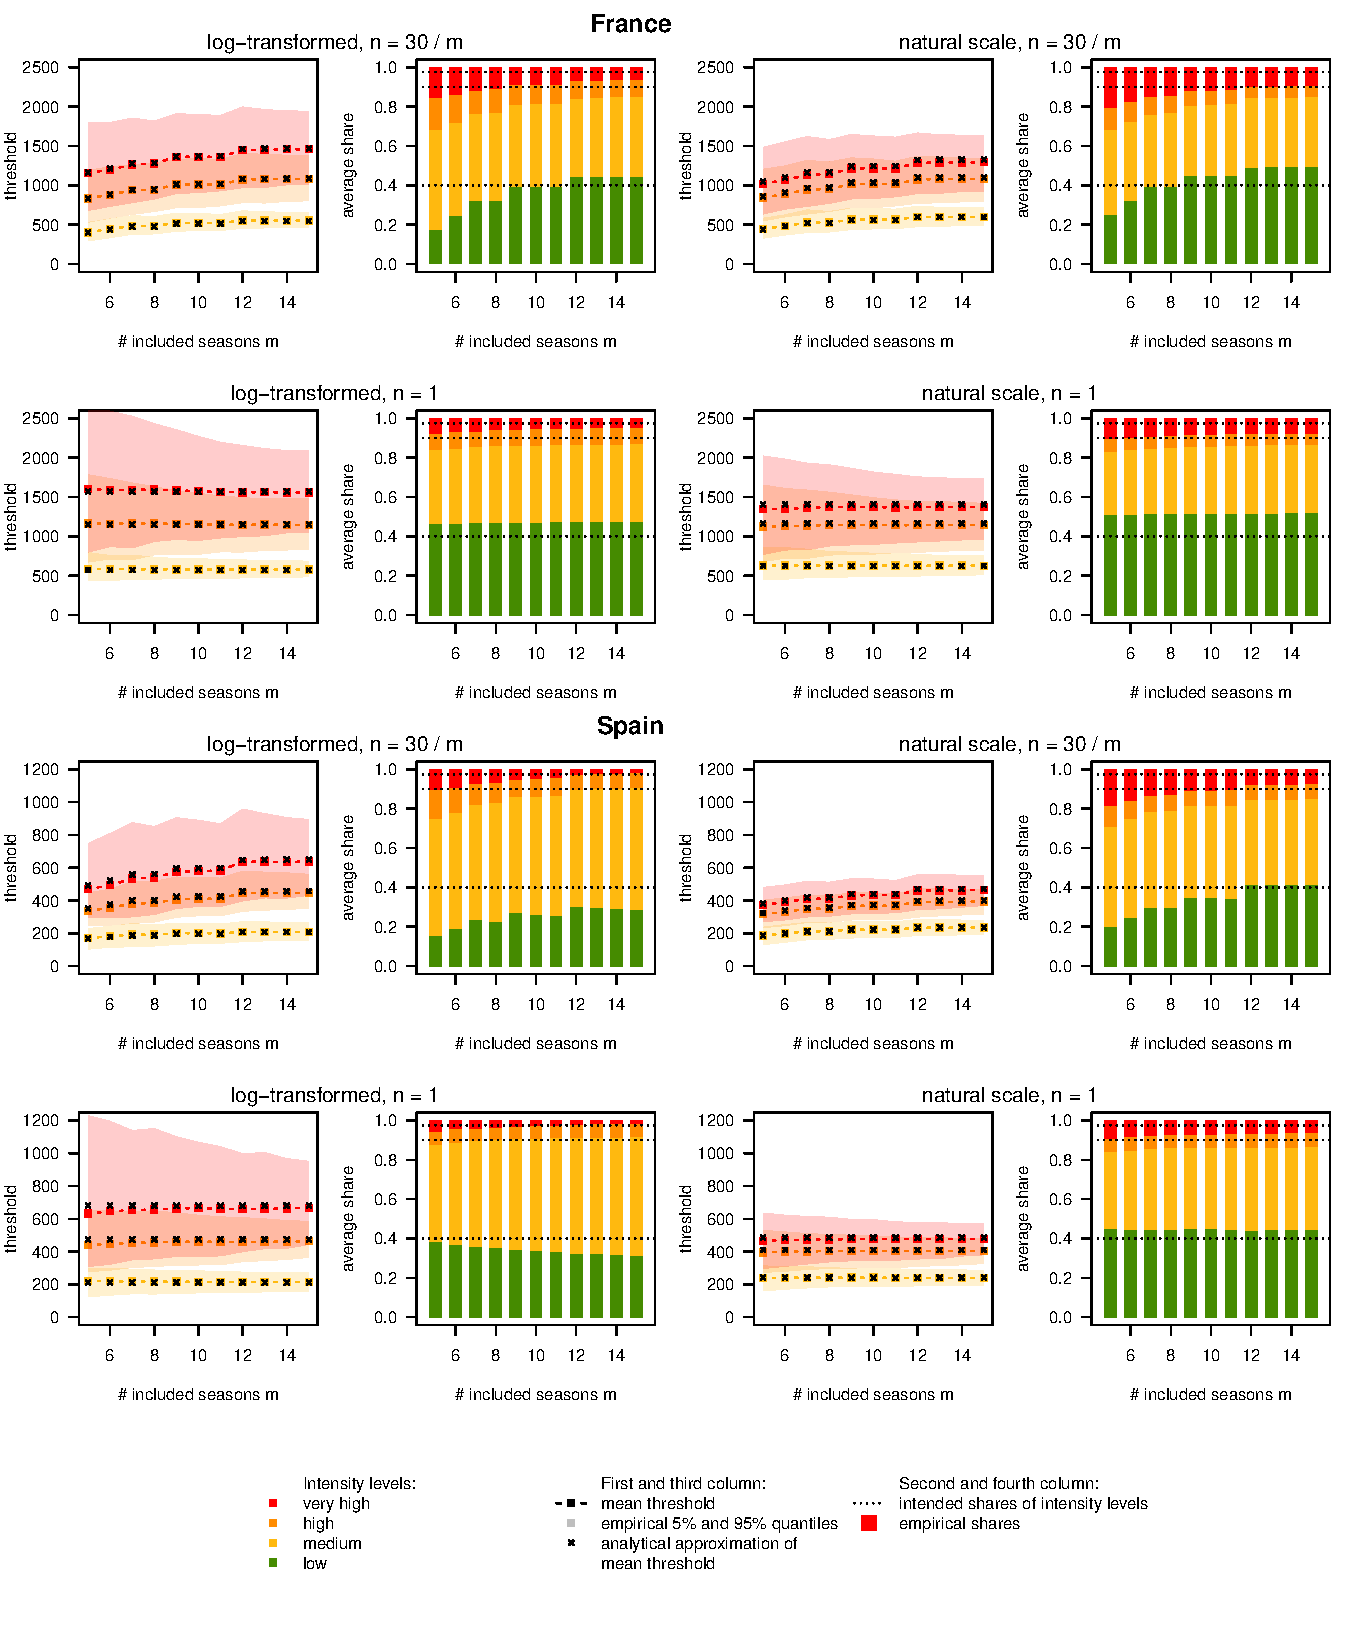
\includegraphics[page=1, width=0.9\textwidth]{figure/plot_results.pdf}
\label{fig:results1}
\end{figure}

\begin{figure}
\includegraphics[page=2, width=0.9\textwidth]{figure/plot_results.pdf}
\caption{Results of bootstrap simulation study for Spain and the United States. First and third column: mean intensity thresholds along with bands delimited by the empirical 5\% and 95\% quantiles. SEcond and fourth columns: resulting average shares of seasons classified as low, medium, high and very high intensity.}
\label{fig:results2}
\end{figure}


\section{Discussion}
\label{sec:discussion}

Mention that also concerns computation of seasonal thresholds.

\section*{Outline of idea}

\begin{itemize}
\item Description of importance: officially embraced by ECDC
\item Describe other approaches, in particular WHO
\item Statistically correct description of what is being done, contract to WHO approach (which only uses peak -- good -- but uses normal rather than log-normal -- not so good. There is a PLOS paper where there is already a kind of combination of the two (WHO with log transformation))
\item Overview of how it is being used in the literature:
\begin{itemize}
\item How much training data was available in each study?
\end{itemize}
\item Simulation study based on bootstrapping of true seasons:
\begin{itemize}
\item Countries: France, Switzerland, some third (European) country? Spain?
\item Important: standardize with time-varying population
\end{itemize}
\end{itemize}

\title{A statistical perspective on the moving epidemic method }
\author{Johannes Bracher}
\maketitle



\bibliographystyle{apalike}
\bibliography{bibliography_mem}
\end{document}